\documentclass[sigconf,screen]{acmart}
\usepackage{tikz}
\usetikzlibrary{positioning, fit, arrows.meta, backgrounds}
\usepackage{enumitem}
\usepackage{float}
\usepackage{graphicx}
\usepackage{microtype}    % nicer justification, helps avoid overflow
\usepackage{url}          % \path{...} allows long paths to break cleanly
\graphicspath{{figures/}}
\setlist{nosep,leftmargin=*}
\settopmatter{printacmref=false}
%% Rights management information.
\setcopyright{none}
\copyrightyear{2026}
\acmYear{2026}
\acmDOI{}
\acmConference[Final Report]{Multimodal Probabilistic Learning of Human Communication}{Spring 2026}{CSCI-535}
\acmBooktitle{Final Report: Multimodal Probabilistic Learning of Human Communication}
\acmISBN{}
\begin{document}
\title{Linguistic-Agnostic Speech Emotion Recognition:\\ A Probing Approach to Acoustic Emotion Encoding}
\subtitle{Multimodal Probabilistic Learning of Human Communication, Final Report}
\author{Nima Kelidari}
\email{kelidari@usc.edu}
\affiliation{%
  \institution{University of Southern California}
  \city{Los Angeles}\state{California}\country{USA}
}
\author{Minoo Ahmadi}
\email{minooahm@usc.edu}
\affiliation{%
  \institution{University of Southern California}
  \city{Los Angeles}\state{California}\country{USA}
}
\author{Chaitanya Parwatkar}
\email{parwatka@usc.edu}
\affiliation{%
  \institution{University of Southern California}
  \city{Los Angeles}\state{California}\country{USA}
}
\author{Xiangxu Lin}
\email{xiangxul@usc.edu}
\affiliation{%
  \institution{University of Southern California}
  \city{Los Angeles}\state{California}\country{USA}
}
\renewcommand{\shortauthors}{Kelidari, Ahmadi, Parwatkar, Lin}
\begin{abstract}
Pretrained speech transformers such as wav2vec~2.0, HuBERT, WavLM, MERT, w2v-BERT, and Whisper achieve state-of-the-art speech-emotion recognition (SER), but it remains unclear whether they predict emotion from paralinguistic delivery or from linguistic content recovered during pretraining. We extend our midterm layer-wise probing study (3 models $\times$ 6 datasets) into a larger framework that combines six frozen encoders with eight datasets across seven languages and a battery of falsification experiments: a lexicon-controlled corpus (CREMA-D), a pooled and leave-one-language-out cross-lingual benchmark (SpeechCraft, Task 9) plus an EN-ZH cross-lingual stress test, low-rank fine-tuning (LoRA) on 30 model$\times$dataset combinations, an attention-based learned layer mixer, BERT representational alignment via CKA / Procrustes / centroid transfer, leave-one-speaker-out evaluation on 42 pairs, gradient-reversal and CCA debiasing, a congruent-vs-incongruent text/voice probe (EMIS), ESC-50 noise augmentation at four SNR levels, and dimensional V/A/D regression on MSP-Podcast. Across these tests, emotion remains decodable from middle-to-late transformer layers in every language we evaluated, frozen probes outperform LoRA on 29 of 30 combinations, three of four self-supervised encoders take a measurable text shortcut while Whisper alone resists it, Whisper is also the most noise-robust encoder (approximately 11\% drop at 0\,dB vs.\ approximately 23 to 30\% for the SSL encoders), and the dimension that depends most on words , valence , is exactly the dimension our probes find hardest. The convergent message is that acoustic emotion structure is recoverable but not exclusively used by every architecture, and that supervised multilingual pretraining produces qualitatively different representations from self-supervised pretraining at every depth we tested.
\end{abstract}
\keywords{speech emotion recognition; layer-wise probing; self-supervised speech models; cross-lingual evaluation; linguistic bias}
\maketitle
\section{Problem Definition}
Speech carries emotion through two channels: linguistic content (what is said) and paralinguistic delivery (how it is said). Pretrained transformers such as wav2vec~2.0~\cite{baevski2020wav2vec}, HuBERT~\cite{hsu2021hubert}, WavLM~\cite{chen2022wavlm}, and Whisper~\cite{radford2023robust} dominate SER benchmarks, yet were trained for speech recognition and therefore encode substantial linguistic structure. If their SER predictions rely on this linguistic content, they will fail under sarcasm, accented speech, low-resource languages, and any condition where lexical meaning and prosody diverge~\cite{wagner2023dawn,triantafyllopoulos2022probing}.
This project asks: (i) \emph{at which depth} of these models is emotion most strongly encoded, (ii) does the depth pattern hold \emph{across languages, speakers, and pretraining paradigms}, and (iii) is the signal that probes pick up \emph{acoustic or lexical}? The midterm answered (i) and (ii) for 3 models on 6 datasets; the final report adds three more encoders, one lexicon-controlled corpus, a large pooled-multilingual benchmark, and four falsification tests that target (iii) directly.
\section{Literature Review}
Prior probing work shows that acoustic features concentrate in early SSL layers while phonetic and word-level information peaks in middle-to-deep layers, with wav2vec~2.0 behaving as an autoencoder in its deepest layers and HuBERT retaining information through iterative clustering~\cite{shah2021audio,pasad2021layer,huo2025iterative}. For SER, Wagner et al.~\cite{wagner2023dawn} showed that fine-tuned wav2vec~2.0/HuBERT retain near-baseline valence accuracy on emotionless TTS of the same transcripts, suggesting heavy lexical reliance; Triantafyllopoulos et al.~\cite{triantafyllopoulos2022probing} confirmed valence (but not arousal/dominance) responds strongly to sentiment-word manipulations. Layer-wise emotion probes have identified middle-layer peaks across multiple SSL models and languages~\cite{singh2023decoding,chiu2025probing,han2025crosslingual}, but the linguistic-acoustic confound has been observed rather than falsified. Our work extends this line by pairing layer-wise probing with controlled falsification (lexicon-fixed corpora, text/voice incongruence, BERT alignment, GRL, CCA projection, noise) to test whether the layer-wise peaks are explained by acoustic structure alone.
\section{Data Description}
We evaluate eight datasets spanning seven languages (Table~\ref{tab:datasets}). The first six are inherited from the midterm and span acted (RAVDESS, EmoDB, SAVEE, AESDD, MESD) and spontaneous (IEMOCAP) speech, four languages, and three recording paradigms. To probe linguistic confounds we add \textbf{CREMA-D}~\cite{cao2014crema}, in which 91 actors speak the same 12 sentences across 6 emotions: any signal recovered must be acoustic. To stress-test cross-lingual transfer we assemble \textbf{SpeechCraft (Task 9)}, a balanced 4-class manifest aggregating 3{,}980 clips across English (n=2{,}546), Spanish (n=576), Greek (n=483), and German (n=375) with labels \{happy, sad, fear, disgust\}; the larger \textasciitilde20k SpeechCraft results (English-only and English+Mandarin pools) are reported separately in \S\ref{sec:enzh}. The full per-class counts are given in Appendix~\ref{app:dataset_counts}.
\begin{table}[h]
\centering
\small
\caption{Datasets used in the final study.}
\label{tab:datasets}
\setlength{\tabcolsep}{4pt}
\begin{tabular}{lllrr}
\toprule
\textbf{Dataset} & \textbf{Lang.} & \textbf{Style} & \textbf{Files} & \textbf{Cls} \\
\midrule
RAVDESS  & English (US)  & Acted        & 1{,}440  & 8 \\
EmoDB    & German        & Acted        & 535      & 7 \\
IEMOCAP  & English (US)  & Spontaneous  & 5{,}460  & 4 \\
SAVEE    & English (UK)  & Acted        & 480      & 7 \\
AESDD    & Greek         & Acted        & 604      & 5 \\
MESD     & Spanish (MX)  & Acted        & 862      & 6 \\
CREMA-D  & English (US)  & Acted (lex.\ fixed) & 7{,}442 & 6 \\
SpeechCraft (Task 9) & 4-lang  & Pooled (4-cls)  & 3{,}980 & 4 \\
\bottomrule
\end{tabular}
\end{table}
\section{Method}
\label{sec:method}
The core idea is straightforward: freeze a pretrained encoder so its weights never change, then test each transformer layer in isolation to measure how much emotion-relevant information it actually carries. If a probe trained on a layer's representation does well, the information is explicitly available there; if it does not, it is either absent or tangled in a way a linear classifier cannot recover. The midterm used this recipe with three Base-sized encoders on six datasets; the final report keeps the same recipe and scales it up across encoder size, encoder family, dataset coverage, and downstream variants designed to test whether the layer-wise signal is acoustic or lexical~\cite{triantafyllopoulos2022probing,shah2021audio,pasad2021layer}.
\subsection{Encoders}
We evaluate six pretrained transformers, all kept fully frozen at every layer for every experiment. To enable fair comparison across pretraining paradigms, every encoder in the final report is a 24-transformer-layer Large variant; this is a deliberate scale-up from the Base-sized encoders used in the midterm. The six span the four major modern paradigms in speech representation learning (Table~\ref{tab:encoders}): contrastive (wav2vec~2.0), masked cluster prediction (HuBERT, WavLM), contrastive plus masked-language-modeling (w2v-BERT), and supervised multilingual transcription (Whisper), with MERT included as a non-speech control because it was pretrained on music. We use only Whisper's encoder; the decoder is never called, so any text-like structure we observe in Whisper's representations is the encoder's own learned structure rather than transcription-head output.

\begin{table}[h]
\centering
\small
\caption{The six 24-layer frozen encoders.}
\label{tab:encoders}
\setlength{\tabcolsep}{4pt}
\begin{tabular}{lll}
\toprule
\textbf{Encoder} & \textbf{Pretraining paradigm} & \textbf{Pretrain data} \\
\midrule
HuBERT      & masked cluster pred.    & 60k h Libri-Light \\
WavLM       & masked clust.\ + denoise & 94k h mixed corpora \\
wav2vec~2.0 & contrastive             & 960 h LibriSpeech \\
w2v-BERT    & contrastive + MLM       & multilingual \\
MERT        & music SSL (control)     & music corpora \\
Whisper     & supervised ASR          & 680k h multilingual \\
\bottomrule
\end{tabular}
\end{table}
\subsection{Feature extraction}
Each audio file is resampled to 16 kHz mono and passed through the frozen encoder with hidden-state output enabled. The SSL encoders take raw waveforms; Whisper takes 80-channel log-mel spectrograms padded or truncated to 30 seconds, after which only the encoder is run. We extract one hidden state from every transformer layer and additionally from the convolutional front-end, which we treat as Layer 0 across all encoders for consistency. Every encoder produces 25 hidden states per utterance: a CNN-front-end Layer 0, plus 24 transformer layers indexed L1 through L24. Each hidden state has shape $(1, T, d)$ where $T$ is the number of time frames and $d$ is the encoder's hidden dimension; we apply mean pooling over $T$ to produce a single fixed-length vector per layer per utterance.
\subsection{Probing classifier}
Pooled vectors are normalized with \texttt{StandardScaler} and passed to a logistic-regression probe trained with 5-fold stratified cross-validation. We pick logistic regression specifically because it is linear: any layer that classifies emotion well under a linear probe is one whose representation makes that information directly available, without needing a non-linear head to recover it. We report mean accuracy and weighted F1 across folds.
\subsection{Probing variants}
\label{sec:probing_variants}
On top of this shared pipeline, we run six variants:
\begin{enumerate}
    \item \emph{Frozen layer-wise probing} (the midterm baseline) maps where emotion peaks across depth on each (encoder, dataset) pair.
    \item \emph{Learned layer mixer} replaces single-layer selection with a softmax attention over all 25 hidden states, trained jointly with the classifier; the resulting attention reveals which depths the model wants to look at.
    \item \emph{Frozen vs.\ LoRA} fine-tunes a low-rank adapter (rank 8, $\alpha{=}16$, dropout 0.1, applied to attention $q$/$v$ projections) at each combination's best probing layer for 10 epochs with AdamW at $2{\times}10^{-4}$.
    \item \emph{BERT representational alignment} compares each speech-encoder layer to BERT~\textsc{base} embeddings of the same utterances using CKA, Procrustes residual, and centroid transfer~\cite{kornblith2019cka}; the same alignment is also computed on IEMOCAP transcripts as a secondary check.
    \item \emph{Leave-one-speaker-out (LOSO)} replaces 5-fold CV with speaker-disjoint folds across 42 (encoder, dataset) pairs to separate genuine emotion encoding from speaker memorization.
    \item \emph{Linguistic-bias falsification} runs three complementary tests: gradient reversal against a sentence-ID head (GRL), CCA projection of speech features orthogonal to text-correlated directions, and an EMIS probe that trains on text-emotion equals audio-emotion and tests on the incongruent condition.
\end{enumerate}
After consultation with the instructor, we added \textbf{CREMA-D}~\cite{cao2014crema} as a lexicon-controlled falsification corpus. Two further extensions sit on top of the same encoders: ESC-50 environmental noise mixed at four SNR levels (20, 10, 5, 0 dB) on MSP-Podcast, and dimensional V/A/D regression with ridge regressors per layer per dimension. The same hidden states feed every variant, so any difference between results is attributable to the head and protocol rather than to the underlying representation.
\subsection{Implementation}
All experiments run in Python with PyTorch and HuggingFace Transformers. Hidden-state extraction runs on an NVIDIA A100 SXM4 40GB GPU; classification uses scikit-learn defaults. Every (encoder, dataset, variant) combination is recorded with its full configuration, per-fold scores, and best-layer summary in the project repository\footnote{\url{https://github.com/Nikelroid/linguistic-agnostic-ser}}; the W\&B project \path{AGSER/linguistic-agnostic-ser} contains all run logs and seeds for full reproducibility.
\begin{figure*}[t]
\centering
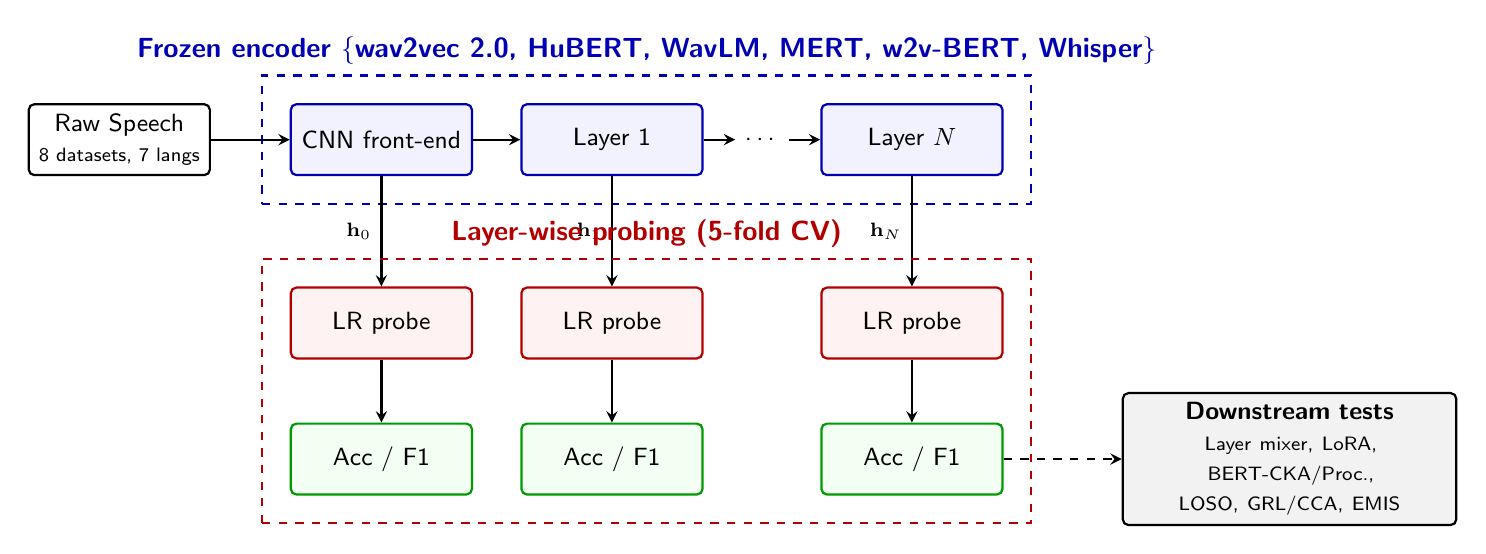
\begin{tikzpicture}[
    >=stealth,
    font=\sffamily\small,
    block/.style={rectangle, draw=black, thick, minimum width=2.3cm, minimum height=0.9cm, align=center, rounded corners=2pt, fill=white},
    frozen/.style={rectangle, draw=blue!70!black, thick, minimum width=2.3cm, minimum height=0.9cm, align=center, rounded corners=2pt, fill=blue!5},
    probe/.style={rectangle, draw=red!70!black, thick, minimum width=2.3cm, minimum height=0.9cm, align=center, rounded corners=2pt, fill=red!5},
    output/.style={rectangle, draw=green!60!black, thick, minimum width=2.3cm, minimum height=0.9cm, align=center, rounded corners=2pt, fill=green!5},
    arrow/.style={->, thick}
]
\node[block] (input) {Raw Speech\\\scriptsize 8 datasets, 7 langs};
\node[frozen, right=1.0cm of input] (cnn) {CNN front-end};
\node[frozen, right=0.6cm of cnn] (layer1) {Layer 1};
\node[right=0.4cm of layer1] (dots) {\dots};
\node[frozen, right=0.4cm of dots] (layerN) {Layer $N$};
\node[draw=blue!70!black, thick, dashed, inner sep=10pt, fit=(cnn) (layer1) (dots) (layerN), label={[text=blue!70!black, font=\sffamily\bfseries]above:Frozen encoder \{wav2vec~2.0, HuBERT, WavLM, MERT, w2v-BERT, Whisper\}}] (model) {};
\draw[arrow] (input) -- (cnn);
\draw[arrow] (cnn) -- (layer1);
\draw[arrow] (layer1) -- (dots);
\draw[arrow] (dots) -- (layerN);
\node[probe, below=1.4cm of cnn] (clf0) {LR probe};
\node[probe, below=1.4cm of layer1] (clf1) {LR probe};
\node[probe, below=1.4cm of layerN] (clfN) {LR probe};
\draw[arrow] (cnn) -- node[left,font=\scriptsize]{$\mathbf{h}_0$} (clf0);
\draw[arrow] (layer1) -- node[left,font=\scriptsize]{$\mathbf{h}_1$} (clf1);
\draw[arrow] (layerN) -- node[left,font=\scriptsize]{$\mathbf{h}_N$} (clfN);
\node[output, below=0.8cm of clf0] (out0) {Acc / F1};
\node[output, below=0.8cm of clf1] (out1) {Acc / F1};
\node[output, below=0.8cm of clfN] (outN) {Acc / F1};
\draw[arrow] (clf0) -- (out0);
\draw[arrow] (clf1) -- (out1);
\draw[arrow] (clfN) -- (outN);
\node[draw=red!70!black, thick, dashed, inner sep=10pt, fit=(clf0) (clf1) (clfN) (out0) (out1) (outN), label={[text=red!70!black, font=\sffamily\bfseries]above:Layer-wise probing (5-fold CV)}] (eval) {};
\node[block, fill=gray!10, right=1.5cm of outN, text width=4cm] (downstream) {\textbf{Downstream tests}\\ \scriptsize Layer mixer, LoRA, BERT-CKA/Proc., LOSO, GRL/CCA, EMIS};
\draw[arrow, dashed] (outN.east) -- (downstream.west);
\end{tikzpicture}
\caption{Unified probing pipeline. The frozen encoder is shared across all six probing variants; only the head and evaluation protocol change.}
\label{fig:methodology_pipeline}
\end{figure*}
\section{Results}
\subsection{Layer-wise probing across six encoders}
\label{sec:probing}
Extending the midterm from three Base-sized encoders to six 24-layer variants confirms its central pattern at substantially larger scale: emotion is decodable across every encoder we tested, the optimal depth concentrates in the middle to late transformer layers on acted speech, and it shifts toward the very early layers on spontaneous conversation. Across all 42 encoder-dataset pairs, acted speech generally peaks somewhere between L7 and L17, while IEMOCAP collapses to the first few layers (L1 to L4) for every encoder. Table~\ref{tab:probe_peak} shows the best-layer accuracy on EmoDB, where most encoders reach their cleanest peaks. What stands out is that Whisper, despite a completely different objective from the SSL models, peaks in the same depth band on most acted corpora; whatever depth represents emotion most cleanly does not seem to depend on whether the encoder was trained for transcription, contrastive prediction, or masked clustering. The full per-(model, dataset) accuracy curves for all 42 combinations are in the project repository under \path{results/}.
\begin{table}[h]
\centering
\small
\caption{Best-layer probing accuracy on EmoDB for each of the six encoders (5-fold stratified CV, 7 emotion classes). Layer 0 is the CNN front-end; transformer layers are L1 through L24.}
\label{tab:probe_peak}
\begin{tabular}{lcc}
\toprule
\textbf{Encoder} & \textbf{Best Layer} & \textbf{Acc} \\
\midrule
HuBERT      & L11 & 0.989 \\
w2v-BERT    & L17 & 0.987 \\
WavLM       & L9  & 0.985 \\
Whisper     & L13 & 0.985 \\
wav2vec~2.0 & L7  & 0.976 \\
MERT        & L7  & 0.961 \\
\bottomrule
\end{tabular}
\end{table}
Two patterns from the midterm reproduce cleanly at this scale. First, the \emph{wav2vec~2.0 deep-layer collapse}: on every acted dataset, wav2vec~2.0 peaks early then drops sharply through the deepest layers, while HuBERT, WavLM, and Whisper hold accuracy further into the stack , consistent with prior work attributing the contrastive objective to word-level prediction overwriting prosody at depth~\cite{huo2025iterative}. Second, the \emph{spontaneous-vs-acted gap}: every encoder peaks much earlier on IEMOCAP than on the acted corpora. WavLM tracks HuBERT closely; MERT (music-pretrained) places its peak in the same middle band as the speech-pretrained SSLs; w2v-BERT peaks deepest of the SSL group (often L17 to L20).
\subsection{SpeechCraft (Task 9, Subtask A): pooled vs.\ LOLO}
\label{sec:exp20}
Task 9 has two subtasks. \textbf{Subtask A} (this section, code in the \texttt{speechcraft} branch under \path{scripts/run_speechcraft.py}) aggregates four European corpora into a 4-class (\{happy, sad, fear, disgust\}) manifest , English $=$ RAVDESS+IEMOCAP+SAVEE, German $=$ EmoDB, Greek $=$ AESDD, Spanish $=$ MESD, normalised to the common 4-class label set , and runs two protocols on each of the six encoders: \emph{pooled} 5-fold CV across languages, and \emph{leave-one-language-out} (LOLO) where one of \{English, German, Greek, Spanish\} is held out entirely from training. \textbf{Subtask B} (\S\ref{sec:enzh}) scales to a larger 20k-style English-only pool and adds a Mandarin partition.

Pooled accuracy saturates: Whisper peaks at 0.949 (L10), HuBERT at 0.947 (L8), and even the weakest encoder (MERT) reaches 0.908 (Table~\ref{tab:exp20-pooled}). LOLO accuracy is uniformly lower and strongly asymmetric (Figure~\ref{fig:exp20}): typologically nearby German held out generalises well (HuBERT 0.952, MERT $\ge$0.88 even at the bottom), Greek and English held out drop to roughly 0.6--0.76, and Spanish held out is the hardest condition for every encoder (HuBERT 0.375, MERT 0.41). The pooled-LOLO gap is therefore a useful proxy for how language-specific the recovered emotion code is for each architecture.
\begin{table}[h]
\centering
\small
\caption{Task 9 Subtask A pooled best-layer accuracy per encoder (4-class, n=3{,}980, 5-fold CV).}
\label{tab:exp20-pooled}
\begin{tabular}{lcc}
\toprule
\textbf{Encoder} & \textbf{Best layer} & \textbf{Acc} \\
\midrule
Whisper     & L10 & 0.949 \\
HuBERT      & L8  & 0.947 \\
WavLM       & L6  & 0.945 \\
w2v-BERT    & L17 & 0.936 \\
wav2vec~2.0 & L8  & 0.922 \\
MERT        & L6  & 0.908 \\
\bottomrule
\end{tabular}
\end{table}
\begin{figure}[h]
\centering
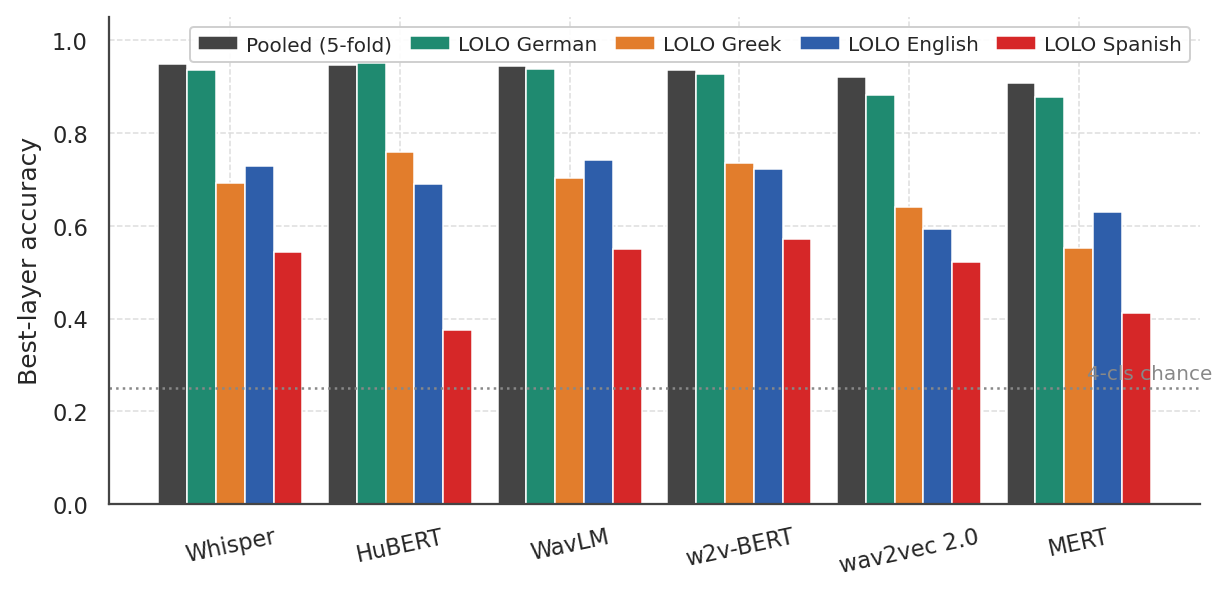
\includegraphics[width=\columnwidth]{speechcraft_summary_bar.png}
\caption{Task 9 Subtask A: per-encoder best-layer accuracy under pooled 5-fold CV (grey) and each leave-one-language-out condition (coloured). German held out is the easy case across the board; Spanish held out is the hard case.}
\label{fig:exp20}
\end{figure}
\subsection{Frozen vs.\ LoRA fine-tuning}
\label{sec:lora}
For each of the 30 (encoder, dataset) combinations across \{RAVDESS, EmoDB, SAVEE, AESDD, MESD\}, a low-rank adapter at the per-combination best layer is fine-tuned and re-probed. The mean best-layer delta (tuned $-$ frozen) is $-0.062$ and the mean over the deepest layer band is $-0.173$; only WavLM/RAVDESS is positive ($+0.003$), and MERT/SAVEE collapses by $-0.144$ (Figure~\ref{fig:lora}). The features the probe needs are already in the frozen encoder, and tuning at a single layer overwrites them more often than it adds; the frozen protocol is competitive with the obvious adaptation baseline.
\begin{figure}[h]
\centering
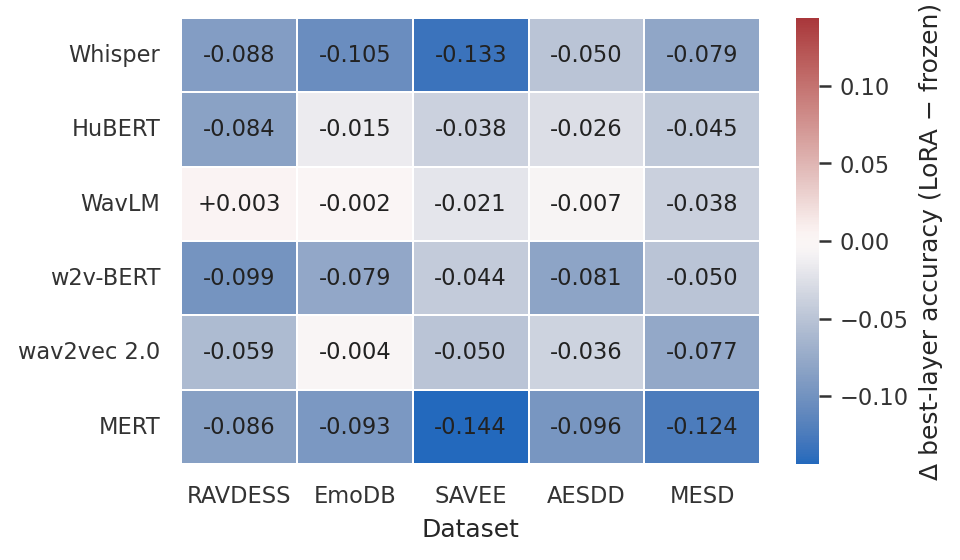
\includegraphics[width=\columnwidth]{lora_delta_heatmap.png}
\caption{Per-layer LoRA-vs-frozen accuracy delta across 30 (encoder, dataset) pairs. Cool = LoRA hurts, warm = LoRA helps. Negative dominates almost everywhere, especially in the deepest layers.}
\label{fig:lora}
\end{figure}
\begin{figure*}[t]
\centering
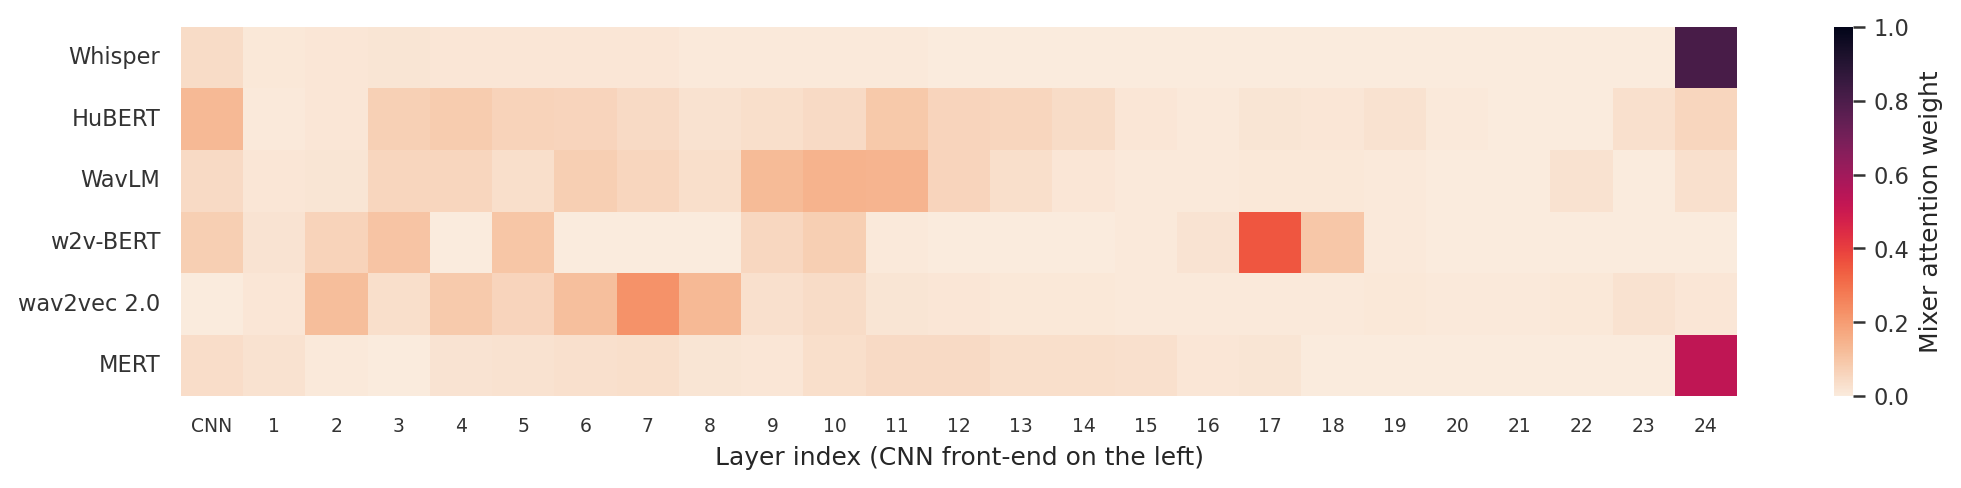
\includegraphics[width=\textwidth]{mixer_attention_heatmap.png}
\caption{Layer-mixer softmax attention weights, averaged across datasets. Whisper concentrates 64\% to 95\% of its attention on L24 across all datasets; the SSL encoders spread attention across layers 4--13. MERT also collapses heavily to L24 on average.}
\label{fig:mixer}
\end{figure*}
\subsection{Learned layer mixer}
\label{sec:mixer}
Replacing single-layer probing with a softmax-attention mixer over all 25 hidden states gives a downstream classifier the freedom to pick its own depth. On the small acted datasets, the mixer mostly under-performs the best single layer (e.g.\ wav2vec~2.0 on RAVDESS: 0.881 vs.\ 0.958), corroborating rather than replacing the per-layer analysis. Two consistent exceptions appear: \emph{IEMOCAP} (mixer beats best layer for 5/6 encoders, gain $+0.02$ to $+0.04$), and \emph{MSP-Podcast} (mixer beats best layer for all 6 encoders, gain $+0.02$ to $+0.06$). Both are spontaneous corpora , consistent with the midterm finding that real conversation does not localize to a single layer cleanly. The attention distribution itself is informative (Figure~\ref{fig:mixer}): \textbf{Whisper concentrates 64\% to 95\% of its attention on the final encoder layer (L24)} across every dataset, while the SSL encoders spread attention over layers 4--13. This is the clearest behavioral signal yet that Whisper's supervised pretraining produces a qualitatively different depth profile from the SSL encoders.
\begin{figure*}[t]
\centering
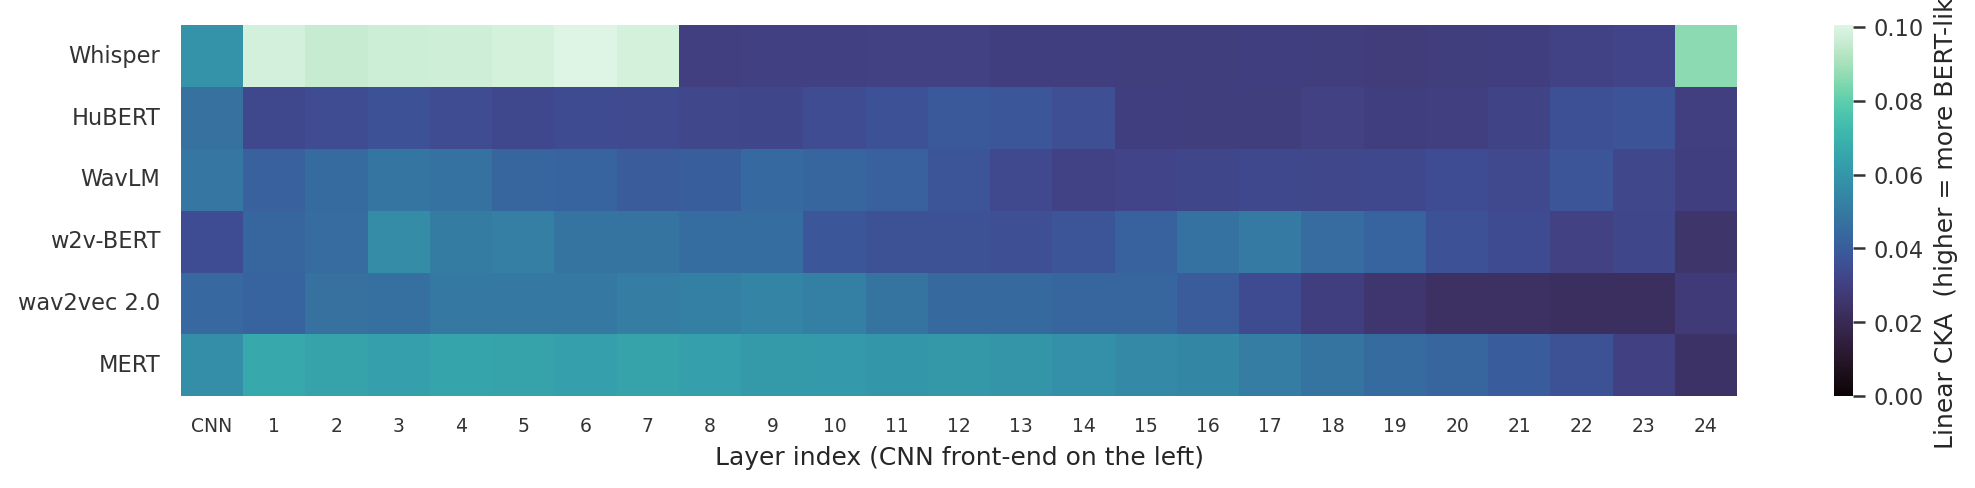
\includegraphics[width=\textwidth]{bert_cka_heatmap.png}
\caption{Linear-CKA alignment between each encoder layer and BERT~\textsc{base} embeddings of the same utterances, averaged across the seven evaluation datasets. Whisper's early encoder layers (1--7) are most BERT-like; SSL encoders spread alignment across the middle band.}
\label{fig:bert}
\end{figure*}
\subsection{BERT representational alignment}
\label{sec:bert-align}
Hidden states from each encoder layer are aligned to BERT~\textsc{base} embeddings of the same utterances using three metrics: linear CKA, Procrustes residual, and centroid transfer~\cite{kornblith2019cka}. Across all six encoders and seven datasets (Figure~\ref{fig:bert}), Procrustes alignment to BERT increases steadily through the middle layers, and \textbf{Whisper's Procrustes alignment grows monotonically toward L24}, peaking on every dataset at the deepest layer (e.g.\ MSP-Podcast 0.861, MESD 0.855, IEMOCAP 0.849). The same encoder-rank holds when the probe operates on \emph{transcripts of the same utterances}: Whisper's CKA reaches 0.392 at L24, the highest value any model attains on the transcript variant. Combined with the layer-mixer behavior in \S\ref{sec:mixer}, this is consistent with Whisper's deep layers carrying more text-like structure than the SSL deep layers.
\subsection{Speaker-independent evaluation (LOSO)}
\label{sec:loso}
Replacing 5-fold CV with leave-one-speaker-out across 42 pairs reveals three patterns:
\begin{itemize}
  \item Speaker-rich datasets retain accuracy: HuBERT/EmoDB drops 0.021 (0.989$\to$0.968 at L11), wav2vec~2.0/EmoDB 0.019, HuBERT/IEMOCAP 0.026.
  \item Speaker-poor datasets collapse: MESD averages 0.30 drop, RAVDESS 0.18, worst MERT/MESD 0.32.
  \item The best layer often shifts \emph{deeper} under LOSO: Whisper/SAVEE L9$\to$L24 ($\Delta=+15$), HuBERT/SAVEE L7$\to$L17, WavLM/SAVEE L6$\to$L18 , so deep layers are more speaker-invariant on small acted corpora.
\end{itemize}
MSP-Podcast is reported separately because all six LOSO probes are only $+0.04$--$+0.06$ above the 0.507 majority-class baseline.
\subsection{CREMA-D: lexicon-controlled probe}
\label{sec:cremad}
CREMA-D~\cite{cao2014crema} fixes the spoken text across all clips (91 actors, 12 carrier sentences, 6 emotions), so any accuracy above the 16.7\% chance line is necessarily acoustic. Figure~\ref{fig:cremad}(a) shows the per-actor accuracy spread for the best (WavLM/L14) probe across the 91 speakers: the mean is 76.1\%, the spread is 45\% to 92\%, and only one outlier actor falls below 50\%. Figure~\ref{fig:cremad}(b) shows the per-encoder best-layer accuracy ranking: WavLM tops at 76.1\%, the rest of the SSL group sits at 73--75\%, and MERT trails at 64.0\%. These numbers are far above chance for every encoder, and the cross-actor variance is moderate, so the layer-wise probe is recovering acoustic emotion content even with the lexical channel held constant.

\begin{figure*}[t]
\centering
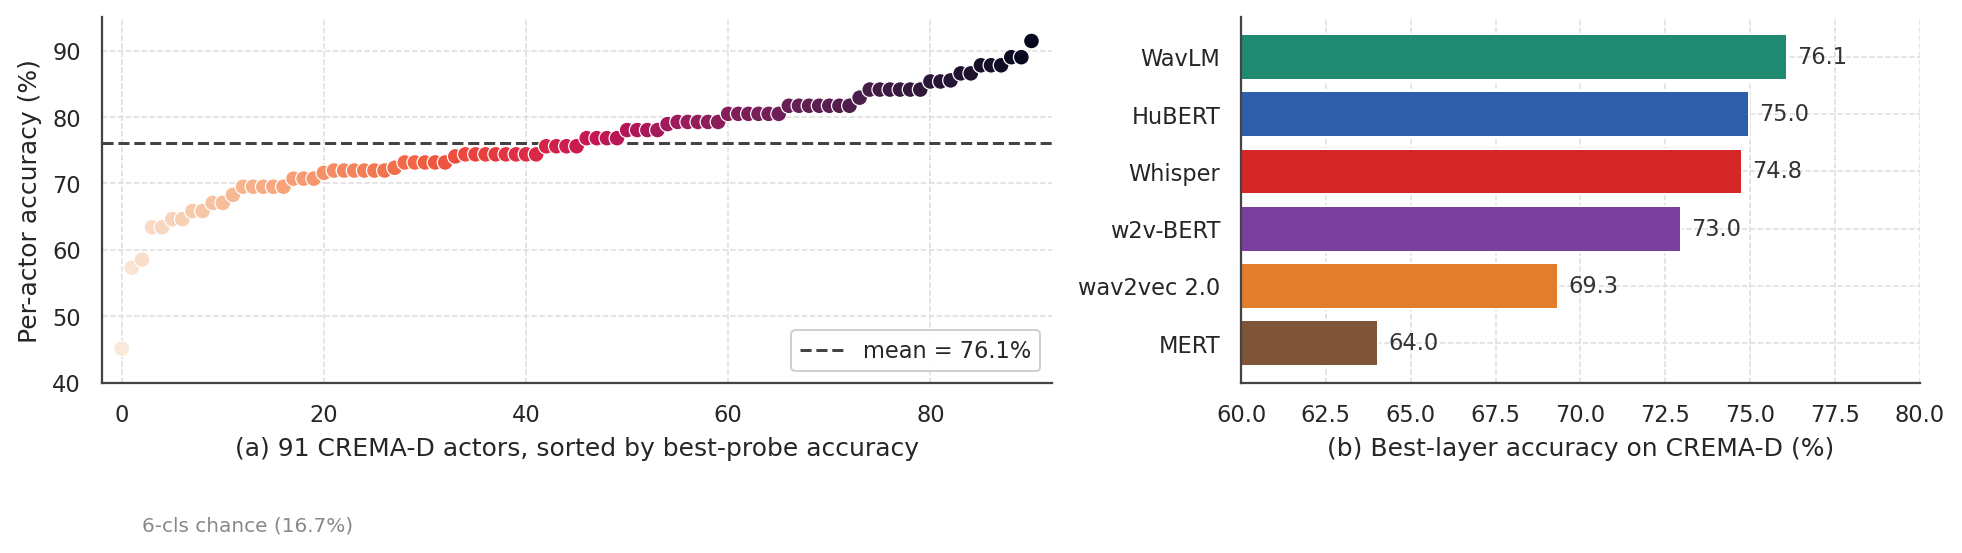
\includegraphics[width=\textwidth]{cremad_per_actor.png}
\caption{CREMA-D, lexicon-controlled probe. \textbf{(a)} Per-actor accuracy across 91 actors, sorted; even the worst actor stays well above chance. \textbf{(b)} Per-encoder best-layer accuracy on CREMA-D.}
\label{fig:cremad}
\end{figure*}

\subsection{Linguistic-bias falsification}
\label{sec:bias}
Three complementary tests target the central question of whether the layer-wise probe is leaning on lexical structure.

\textbf{(a) Congruent vs.\ incongruent EMIS.} We train a 4-class probe on EMIS\textsubscript{congruent} clips (text emotion = audio emotion) and test on EMIS\textsubscript{incongruent} clips (text $\neq$ audio). We then report \emph{text bias} = $\textit{proxy\_acc} - \textit{target\_acc}$, where \emph{proxy} predicts the text emotion and \emph{target} the audio emotion; positive values indicate the probe took a lexical shortcut. The full layer-wise trajectory (Figure~\ref{fig:emis-traj}) is decisive: all three SSL encoders start audio-grounded (text bias $\approx -0.6$ at the CNN front-end) but climb steeply through the middle layers, with HuBERT and WavLM crossing zero around L13 and peaking near $+0.7$ at L20; wav2vec~2.0 reaches the shortcut even faster, crossing zero by L8. \textbf{Whisper alone never crosses zero}: its trajectory rises but plateaus around $-0.2$ even at L24. The peak per-encoder values on the explicit slice (Table~\ref{tab:emis}) confirm the picture.
\begin{table}[h]
\centering
\small
\caption{EMIS text bias on the explicit slice (peak layer per encoder). Positive = probe predicts the text emotion.}
\label{tab:emis}
\begin{tabular}{lccc}
\toprule
\textbf{Encoder} & \textbf{Layer} & \textbf{target acc} & \textbf{text bias} \\
\midrule
HuBERT      & L20 & 0.107 & $+0.717$ \\
wav2vec~2.0 & L15 & 0.123 & $+0.665$ \\
WavLM       & L20 & 0.146 & $+0.613$ \\
Whisper     & L24 & 0.524 & $-0.191$ \\
\bottomrule
\end{tabular}
\end{table}

\begin{figure}[h]
\centering
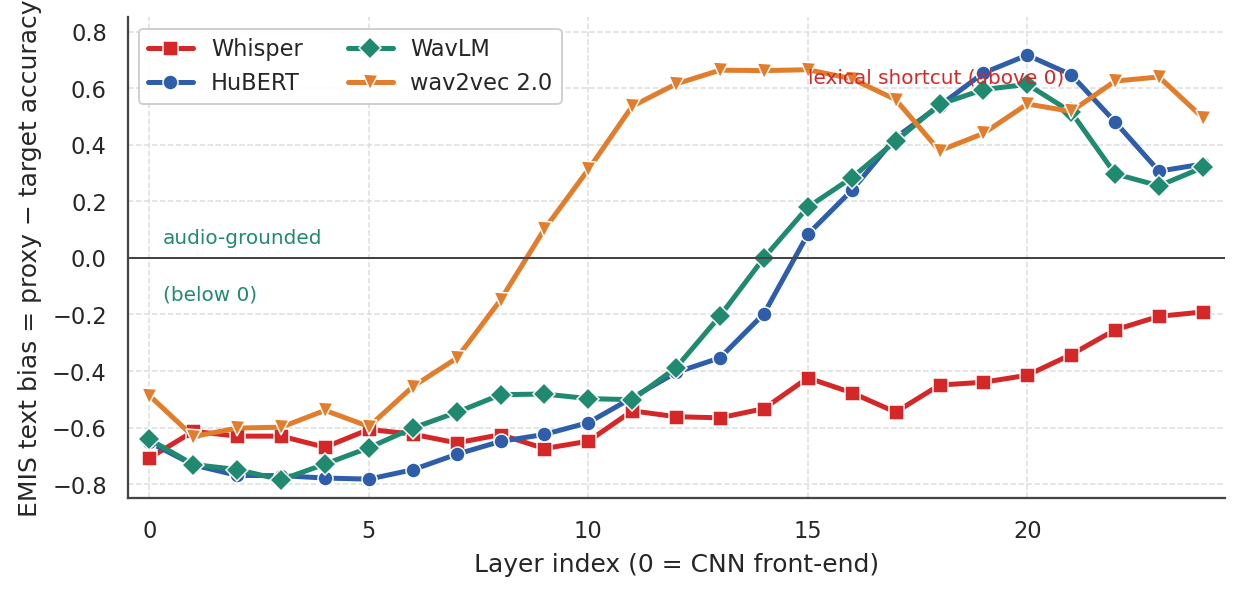
\includegraphics[width=\columnwidth]{emis_text_bias_trajectory.png}
\caption{EMIS text-bias trajectory across all 25 layers. SSL encoders cross from audio-grounded (negative) into the lexical-shortcut regime (positive) by mid-depth; Whisper plateaus and stays negative throughout.}
\label{fig:emis-traj}
\end{figure}
\textbf{(b) Annotator-disagreement ceiling on IEMOCAP.} We split IEMOCAP into 1{,}308 unanimously-labeled clips and 4{,}152 clips with $\geq 1$ annotator disagreement, and probe each subset. All six encoders show a high-vs-low-agreement gap of $+0.145$ to $+0.191$ at the peak layer (mean $+0.169$), confirming that the 65--70\% IEMOCAP ceiling reported in the midterm reflects label noise rather than a probe limitation.
\textbf{(c) Adversarial removal (GRL) and CCA projection.} On EMIS we attempt to remove the text shortcut at inference time. A two-regime baseline reveals it most clearly: when probes are trained on RAV+SAV (no text/emotion correlation), text bias is negative for all four encoders (HuBERT L20: $-0.246$; wav2vec~2.0 L14: $-0.086$; WavLM L20: $-0.268$; Whisper L24: $-0.251$). When the same probes are trained on EMIS\textsubscript{congruent} (text and emotion correlate), three of the four flip strongly positive (HuBERT $+0.928$, wav2vec~2.0 $+0.926$, WavLM $+0.850$); \emph{Whisper alone resists} ($+0.003$). Both attempted post-hoc fixes leave only small Δbias at safe operating points: GRL ($\lambda \le 1$) gives at most $-0.082$ to $-0.113$; CCA projection of the top-$k$ BERT-correlated directions gives at most $-0.018$. The shortcut is robust to standard linear and adversarial debiasing on top of a frozen encoder.
\subsection{ESC-50 noise robustness across 7 datasets}
\label{sec:noise}
TASK 1/2/8 mixes ESC-50 environmental sounds at four SNR levels (20, 10, 5, 0\,dB) into all six encoder $\times$ all seven datasets in our study. Figure~\ref{fig:noise} reports the per-(encoder, dataset) clean-vs-0\,dB accuracy drop across the full 6$\times$7 grid; the encoder mean drops are summarised in Table~\ref{tab:noise}.

Whisper's lead is not a single-dataset artifact: it is the most resilient encoder on \emph{every} one of the 7 datasets (drop range 3.4\% on MSP-Podcast to 20.9\% on SAVEE). The SSL encoders cluster at 22--30\% mean drop, with WavLM the worst case on RAVDESS (43\%) and SAVEE (52\%) , the same datasets where speaker count is small and the acted prosody is most stylized. Two cross-cutting patterns: (i) MSP-Podcast and EmoDB are the easiest noise conditions for every encoder (clean accuracies are already high, fold sizes large, and absolute drops small), and (ii) RAVDESS, SAVEE, and MESD are the hardest, indicating the noise-robustness gap between Whisper and the SSL encoders is widest on small acted corpora where prosody dominates over content. The optimal layer also drifts slightly deeper as SNR worsens for HuBERT (e.g.\ clean L8.6 $\to$ 0\,dB L12.4 on average) but stays roughly invariant for Whisper.

\begin{figure}[h]
\centering
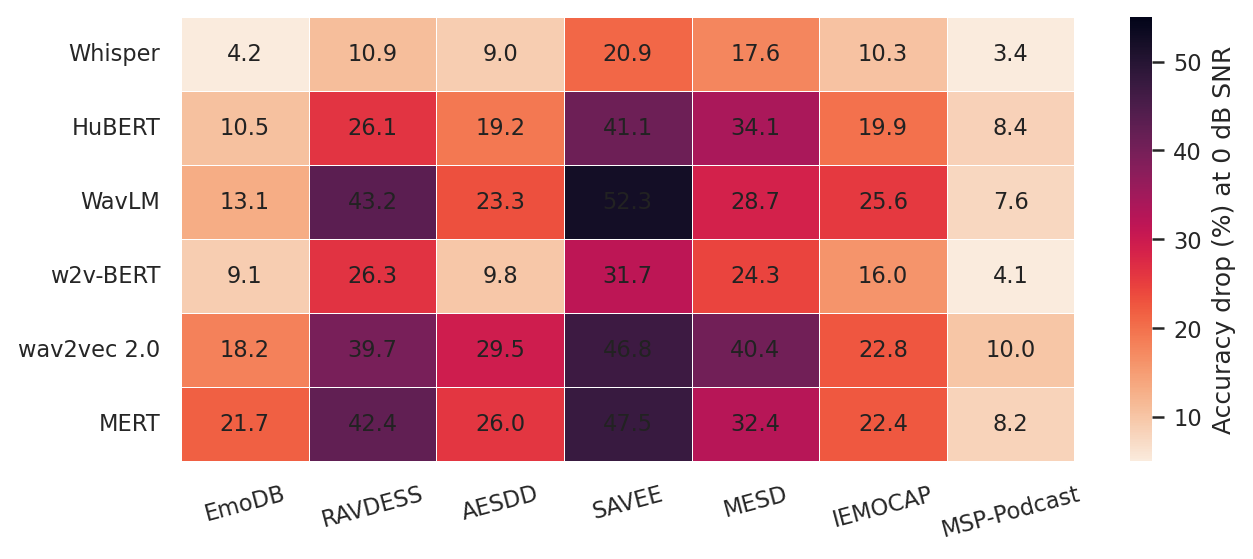
\includegraphics[width=\columnwidth]{noise_drop_heatmap.png}
\caption{ESC-50 noise robustness: per-(encoder, dataset) accuracy drop (\%) at 0\,dB SNR vs.\ clean (Drive: TASK 1/2/8). Whisper's row is the lightest across every dataset.}
\label{fig:noise}
\end{figure}

\begin{table}[h]
\centering
\small
\caption{ESC-50 noise robustness: mean per-encoder accuracy drop at 0\,dB averaged across the 7 datasets in Figure~\ref{fig:noise}. Source: Drive TASK 1/2/8.}
\label{tab:noise}
\begin{tabular}{lc}
\toprule
\textbf{Encoder} & \textbf{Mean drop at 0\,dB} \\
\midrule
Whisper      & $10.9\%$ \\
w2v-BERT     & $16.9\%$ \\
HuBERT       & $22.8\%$ \\
WavLM        & $27.7\%$ \\
MERT         & $28.7\%$ \\
wav2vec~2.0  & $29.6\%$ \\
\bottomrule
\end{tabular}
\end{table}
\begin{figure*}[t]
\centering
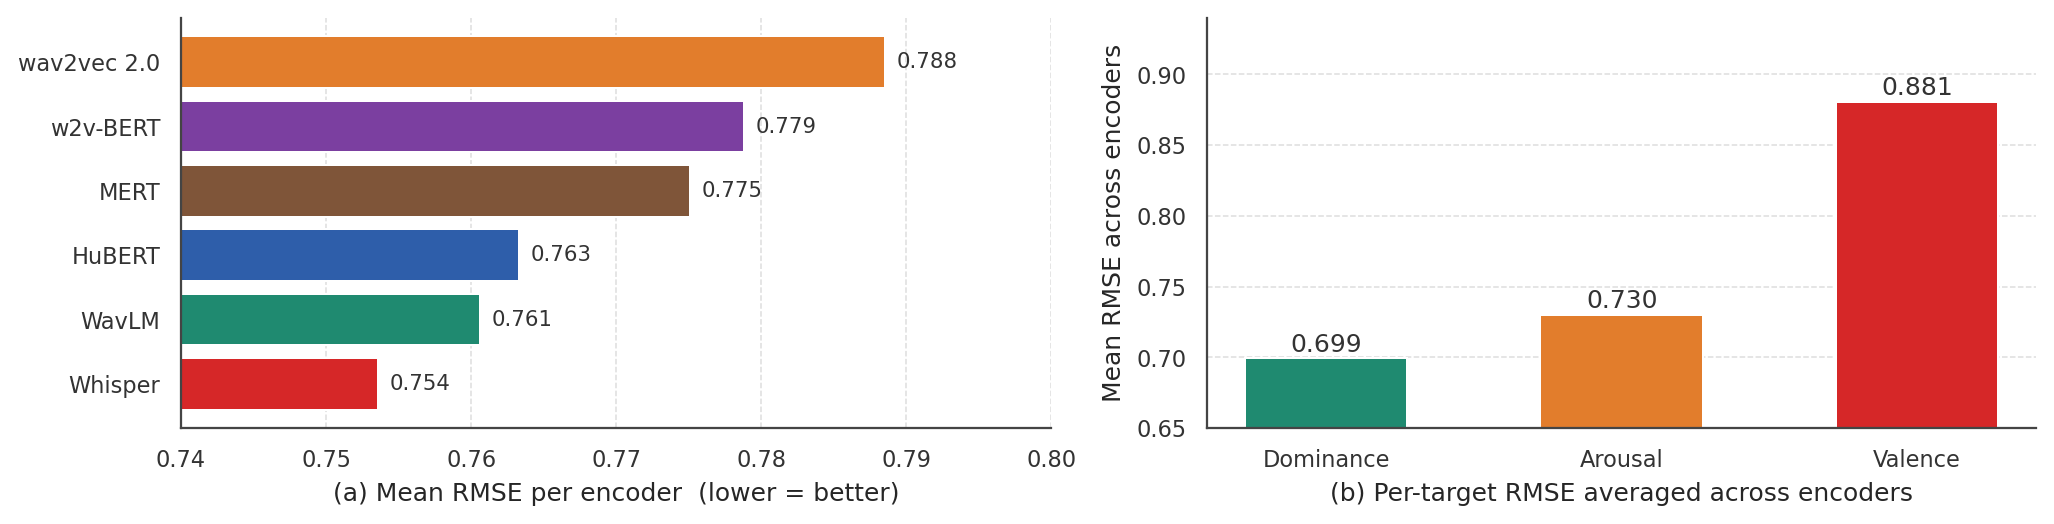
\includegraphics[width=\textwidth]{vad_rmse.png}
\caption{V/A/D regression on MSP-Podcast (ridge probes per layer per dimension). \textbf{(a)} Mean RMSE per encoder; Whisper is best, wav2vec~2.0 worst. \textbf{(b)} Averaged across encoders, valence is by far the hardest dimension , the same dimension prior work attributes to lexical content.}
\label{fig:vad}
\end{figure*}
\subsection{Dimensional V/A/D regression (Tasks 10--12)}
\label{sec:vad}
On MSP-Podcast we replace the 4-class probe with three layer-wise ridge regressors targeting valence (EmoVal), arousal (EmoAct), and dominance (EmoDom). Three Drive analyses give a coherent picture and a clean justification for why valence is the hardest of the three.

\textbf{Clean V/A/D (Drive: TASK 10 statistical analysis).} Averaging RMSE across the six encoders, the per-target ranking is unambiguous (Figure~\ref{fig:vad}b):
\begin{itemize}
  \item EmoDom (dominance): mean RMSE \textbf{0.699}, range 0.690--0.715.
  \item EmoAct (arousal): mean RMSE \textbf{0.730}, range 0.722--0.741.
  \item EmoVal (valence): mean RMSE \textbf{0.881}, range 0.808--0.958 , the only target where any encoder breaks 0.95 RMSE, and every encoder's worst RMSE is on valence.
\end{itemize}
Whisper achieves the lowest mean RMSE (0.754) and wav2vec~2.0 the highest (0.789); all six encoders place their best EmoDom layer at moderate depth (Whisper L12, HuBERT L3, WavLM L3, MERT L8, w2v-BERT L17, wav2vec~2.0 L5). This is the dimension-level analogue of the EMIS finding (\S\ref{sec:bias}): valence is the affective dimension prior work~\cite{wagner2023dawn,triantafyllopoulos2022probing} attributes to lexical content, and it is exactly the dimension every probe finds hardest, while arousal and dominance , which depend on prosodic cues like pitch range and loudness , come out comfortably better across all encoders.

\textbf{Noisy V/A/D (Drive: TASK 11 statistical analysis).} Re-running the same regression on ESC-50-mixed audio at four SNR levels confirms Whisper's noise advantage from \S\ref{sec:noise}. The 0\,dB-vs-clean RMSE delta per encoder (lower = more resilient): Whisper $+0.028$, w2v-BERT $+0.042$, MERT $+0.060$, HuBERT $+0.061$, WavLM $+0.062$, wav2vec~2.0 $+0.071$. The ordering is identical to the noise-robust ordering of the 4-class classifier in \S\ref{sec:noise}, suggesting noise robustness is a property of the encoder rather than of the downstream head.

\textbf{V/A/D-as-features (Drive: TASK 12 statistical analysis).} Treating $\{$valence, arousal, dominance, gender$\}$ as features for a 4-class MSP-Podcast emotion classifier ($n{=}67{,}929$) ranks the four features by mutual information: valence \textbf{MI 0.341} (normalized 1.00), arousal MI 0.197 (norm.\ 0.58), dominance MI 0.200 (norm.\ 0.59), and gender MI 0.015 (norm.\ 0.04). A Random Forest on these four features alone reaches accuracy 0.73 / macro-F1 0.65 (MLP 0.73/0.64, Logistic Regression 0.73/0.58); neutral and happy dominate recall (0.87/0.59), while sad collapses (RF recall 0.25, LR recall 0.06) because sad is the minority class ($\sim$6\%). Tasks 10--12 together paint a single picture: valence is the hardest dimension to recover from acoustics, but \emph{when} you can recover it, it is also the most informative single feature for downstream categorical emotion , precisely because it is the dimension that absorbs the lexical-content variance the EMIS test (\S\ref{sec:bias}) flags as a shortcut.

\subsection{SpeechCraft (Task 9, Subtask B): EN--ZH stress test}
\label{sec:enzh}
Subtask B scales to the larger SpeechCraft compilation and runs four protocols on HuBERT, WavLM, Whisper, and (English-pool only) wav2vec~2.0; per-protocol best-layer weighted F1 is summarised in Table~\ref{tab:task9}.

\begin{table}[h]
\centering
\small
\caption{Task 9 (SpeechCraft) best-layer weighted F1 across four protocols.}
\label{tab:task9}
\setlength{\tabcolsep}{4pt}
\begin{tabular}{lcccc}
\toprule
\textbf{Encoder} & \textbf{EN pool} & \textbf{EN+ZH pool} & \textbf{EN$\to$ZH} & \textbf{ZH$\to$EN} \\
\midrule
Whisper      & 0.776 (L9)  & 0.523 (L22) & 0.291 (L20) & 0.317 (L11) \\
HuBERT       & 0.767 (L11) & 0.485 (L9)  & 0.293 (L8)  & 0.308 (L15) \\
WavLM        & 0.764 (L9)  & 0.513 (L7)  & 0.295 (L7)  & 0.308 (L15) \\
wav2vec~2.0  & 0.723 (L8)  & ---         & ---         & ---         \\
\bottomrule
\end{tabular}
\end{table}

The four protocols expose three findings:
\begin{itemize}
  \item \textbf{Within-English saturation.} On the EN-only pool, all four encoders cluster between weighted F1 0.72 and 0.78 , a tight $\le$0.06 spread that mirrors the saturation we saw on the smaller European pool in \S\ref{sec:exp20}.
  \item \textbf{Adding Mandarin to the training pool nearly halves accuracy.} EN+ZH pooled drops every encoder to weighted F1 0.49--0.52 , a $\sim$0.25 absolute collapse from the EN-only pool, indicating English and Mandarin do not share the same layer-wise emotion subspace and the linear probe cannot fit both at once with a single head.
  \item \textbf{Cross-lingual transfer collapses to chance in both directions.} Train-EN test-ZH and train-ZH test-EN both peak at weighted F1 0.29--0.32 , only marginally above the 4-class chance line of 0.25. The symmetry across directions rules out a ``Mandarin is harder'' explanation: it is the EN--ZH \emph{boundary} itself that the layer-wise emotion code does not cross.
\end{itemize}
The Task 9 results bound the cross-lingual claim from \S\ref{sec:exp20}: the layer-wise emotion code transfers cleanly inside the Indo-European family but not across the Indo-European/Sino-Tibetan boundary, even when over 1000 Mandarin training clips are available.

\section{Conclusions}
Across six encoders, eight datasets, seven languages, and the falsification battery above, three claims survive every test we ran.

\textbf{(C1) Emotion lives in middle-to-late transformer layers.} All six encoders place the emotion peak in the same depth band on every acted dataset and at the very early layers on spontaneous IEMOCAP; CREMA-D reproduces this depth pattern even when no lexical signal is available.

\textbf{(C2) The layer-wise signal generalizes inside a language family but not across it.} Pooled European SpeechCraft saturates near 0.94 across encoders; LOLO transfer is asymmetric (German held out generalizes; English held out does not). Speaker leakage is small on speaker-rich corpora ($\le 0.03$ drop) but severe on small ones (MESD $\sim 0.30$). Adding Mandarin (Task 9) collapses EN$\leftrightarrow$ZH cross-lingual transfer to 0.29--0.32 weighted F1, marginally above chance. LoRA fine-tuning at the best layer hurts on 29 of 30 combinations , features are already in the frozen encoder.

\textbf{(C3) SSL encoders take a lexical shortcut when one is offered; Whisper does not, and is also the most noise-robust.} The EMIS test gives HuBERT, wav2vec~2.0, WavLM text-bias $+0.61$ to $+0.72$ at deep layers; Whisper L24 inverts to $-0.19$. The two-regime baseline confirms it: three SSL encoders flip from $-0.25$ to $+0.85$--$+0.93$ when the training set offers a text shortcut; Whisper stays at $+0.003$. BERT alignment and the layer mixer agree , Whisper concentrates both at L24, the same depth where EMIS shows it remains audio-grounded. Whisper additionally dominates noise robustness ($\sim$11\% drop at 0\,dB vs.\ 23 to 30\% for SSL) and dimensional-regression noise resilience ($\Delta\text{RMSE}=+0.028$ vs.\ $+0.04$--$+0.07$). On valence , the dimension that depends most on words , every encoder still does worst, exactly as prior work predicts. Standard adversarial and projection-based debiasing do not remove the SSL shortcut at any safe operating point.

\noindent The actionable take-away is narrow but robust: probes that report layer-wise emotion accuracy on small acted corpora should be paired with at least one falsification test (lexicon control, EMIS, noise, dimensional V/A/D) before the result is read as ``the model hears emotion in the voice''. The same probe accuracy can be reached two different ways, and our experiments separate them.

\section{Team Contributions}
\textbf{Nima Kelidari.} Built the Slurm-based experiment pipeline and extended the probing grid to six encoders by adding WavLM, w2v-BERT, and MERT. Built and ran the ESC-50 noise-augmentation pipeline at four SNR levels (\S\ref{sec:noise}, Drive: TASK 1/2/8) and the MSP-Podcast spontaneous-speech pipeline; led the V/A/D dimensional-regression track end-to-end (\S\ref{sec:vad}, Drive: TASK 10/11/12). Co-authored the proposal, led the literature review, coordinated report formatting and figure/table styling; ran roughly 360 frozen-layer experiments.

\textbf{Minoo Ahmadi.} Built LOSO evaluation on the frozen probing pipeline (\S\ref{sec:loso}). Gained access to the EMIS dataset and implemented the sentence-stratified text-bias diagnostic on congruent/incongruent clips (\S\ref{sec:bias}); also built the IEMOCAP annotator-disagreement diagnostic. Co-authored the proposals; produced the GRL adversarial and CCA-projection debiasing experiments and the corresponding summary plots and READMEs.

\textbf{Chaitanya Parwatkar.} Built the original layer-wise probing pipeline (hidden-state extraction, mean pooling, \texttt{StandardScaler} + 5-fold logistic regression); ran the BERT alignment experiments via CCA/CKA/Procrustes/centroid transfer; built the learned layer mixer with softmax attention over 25 hidden states; ran LoRA across the 30 (encoder, dataset) combinations; added CREMA-D probing as the cleanest fixed-lexicon test. Wrote the original Method/Results/Cross-Model-Correlation sections of the midterm.

\textbf{Xiangxu Lin.} Compiled the SpeechCraft Task 9 Subtask A benchmark on the \texttt{speechcraft} branch , pooled 5-fold and leave-one-language-out across six encoders on a balanced 4-class European pool (\S\ref{sec:exp20}). Extended Task 9 with Subtask B: large-scale EN-only and EN+ZH pooled protocols plus EN$\to$ZH / ZH$\to$EN cross-lingual conditions on four encoders (\S\ref{sec:enzh}, Table~\ref{tab:task9}). Initiated the midterm report and wrote the original Data Description section.

\bibliographystyle{ACM-Reference-Format}
\begin{thebibliography}{20}
\bibitem{wagner2023dawn}
J.~Wagner et al., ``Dawn of the transformer era in speech emotion recognition: Closing the valence gap,'' \textit{IEEE TPAMI}, vol.~45, no.~9, pp.~10745--10759, 2023.
\bibitem{triantafyllopoulos2022probing}
A.~Triantafyllopoulos et al., ``Probing speech emotion recognition transformers for linguistic knowledge,'' in \textit{Proc.\ INTERSPEECH}, 2022, pp.~146--150.
\bibitem{baevski2020wav2vec}
A.~Baevski et al., ``wav2vec~2.0: A framework for self-supervised learning of speech representations,'' in \textit{Proc.\ NeurIPS}, 2020, pp.~12449--12460.
\bibitem{hsu2021hubert}
W.-N.~Hsu et al., ``HuBERT: Self-supervised speech representation learning by masked prediction of hidden units,'' \textit{IEEE/ACM TASLP}, vol.~29, pp.~3451--3460, 2021.
\bibitem{radford2023robust}
A.~Radford et al., ``Robust speech recognition via large-scale weak supervision,'' in \textit{Proc.\ ICML}, 2023, pp.~28492--28518.
\bibitem{chen2022wavlm}
S.~Chen et al., ``WavLM: Large-scale self-supervised pretraining for full-stack speech processing,'' \textit{IEEE J.\ Selected Topics in Signal Processing}, vol.~16, no.~6, pp.~1505--1518, 2022.
\bibitem{li2023mert}
Y.~Li et al., ``MERT: Acoustic music understanding model with large-scale self-supervised training,'' \textit{arXiv:2306.00107}, 2023.
\bibitem{chung2021w2v}
Y.-A.~Chung et al., ``w2v-BERT: Combining contrastive learning and masked language modeling for self-supervised speech pre-training,'' in \textit{Proc.\ ASRU}, 2021, pp.~244--250.
\bibitem{shah2021audio}
J.~Shah et al., ``What all do audio transformer models hear? Probing acoustic representations for language delivery and its structure,'' \textit{arXiv:2101.00387}, 2021.
\bibitem{pasad2021layer}
A.~Pasad, J.-C.~Chou, and K.~Livescu, ``Layer-wise analysis of a self-supervised speech representation model,'' in \textit{Proc.\ ASRU}, 2021, pp.~914--921.
\bibitem{huo2025iterative}
R.~Huo and E.~Dunbar, ``Iterative refinement, not training objective, makes HuBERT behave differently from wav2vec~2.0,'' in \textit{Proc.\ INTERSPEECH}, 2025.
\bibitem{singh2023decoding}
A.~Singh and A.~Gupta, ``Decoding emotions: A comprehensive multilingual study of speech models for speech emotion recognition,'' \textit{arXiv:2308.08713}, 2023.
\bibitem{chiu2025probing}
A.~Y.~F.~Chiu et al., ``A large-scale probing analysis of speaker-specific attributes in self-supervised speech representations,'' \textit{arXiv:2501.05310}, 2025.
\bibitem{han2025crosslingual}
Z.~Han et al., ``Cross-lingual speech emotion recognition: Humans vs.\ self-supervised models,'' in \textit{Proc.\ ICASSP}, 2025.
\bibitem{cao2014crema}
H.~Cao et al., ``CREMA-D: Crowd-sourced emotional multimodal actors dataset,'' \textit{IEEE Trans.\ Affective Computing}, vol.~5, no.~4, pp.~377--390, 2014.
\bibitem{kornblith2019cka}
S.~Kornblith, M.~Norouzi, H.~Lee, and G.~Hinton, ``Similarity of neural network representations revisited,'' in \textit{Proc.\ ICML}, 2019, pp.~3519--3529.
\bibitem{livingstone2018ravdess}
S.~R.~Livingstone and F.~A.~Russo, ``The Ryerson Audio-Visual Database of Emotional Speech and Song (RAVDESS),'' \textit{PLOS ONE}, vol.~13, no.~5, 2018.
\bibitem{busso2008iemocap}
C.~Busso et al., ``IEMOCAP: Interactive emotional dyadic motion capture database,'' \textit{Language Resources and Evaluation}, vol.~42, no.~4, pp.~335--359, 2008.
\end{thebibliography}
\appendix
\section{Per-class counts (six base datasets, CREMA-D, Task 9)}
\label{app:dataset_counts}
The original six datasets follow the midterm Appendix~A counts: RAVDESS (192 neutral; 384 each for calm, angry, disgust, fearful, happy, sad, surprised), EmoDB (127/81/79/71/69/62/46 across angry, bored, neutral, happy, fearful, sad, disgust), IEMOCAP (1{,}708 neutral, 1{,}636 happy, 1{,}103 angry, 1{,}084 sad), SAVEE (120 neutral; 60 each for the remaining six classes), AESDD ($\sim$121 per emotion), and MESD ($\sim$144/143 per emotion). CREMA-D contributes 7{,}442 utterances from 91 actors saying the same 12 sentences across 6 emotions (anger, disgust, fear, happy, neutral, sad); per-actor and per-sentence accuracies for our best probe live in the Task 9 / CREMA-D directories of the project repository. The Task 9 balanced subset breaks down as English 2{,}546, German 375, Greek 483, Spanish 576, with class counts: happy 831, sad 1{,}768, fear 701, disgust 680.
\section{Extended Task 9 Subtask A figures}
\label{app:exp20-figs}
\begin{figure*}[t]
\centering
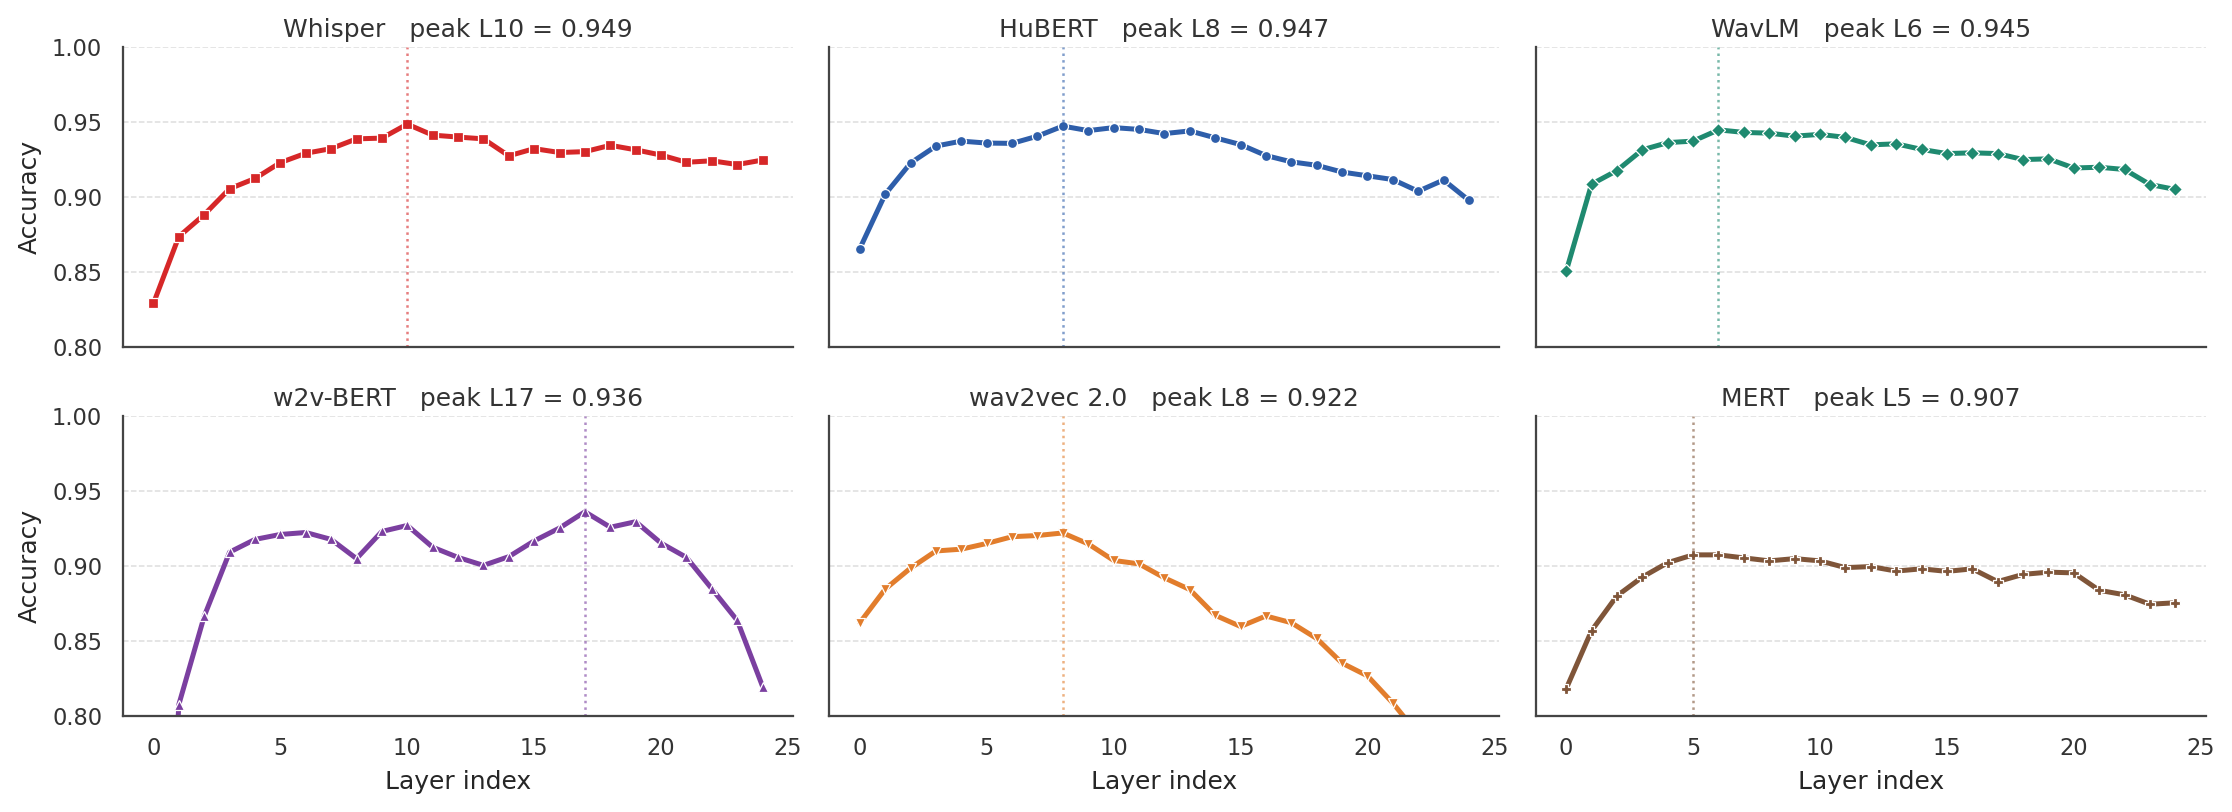
\includegraphics[width=\textwidth]{speechcraft_pooled_grid.png}
\caption{Task 9 Subtask A pooled per-encoder layer-wise accuracy curves; vertical dotted line marks each encoder's peak layer.}
\label{fig:exp20-pooled-grid}
\end{figure*}
\begin{figure}[h]
\centering
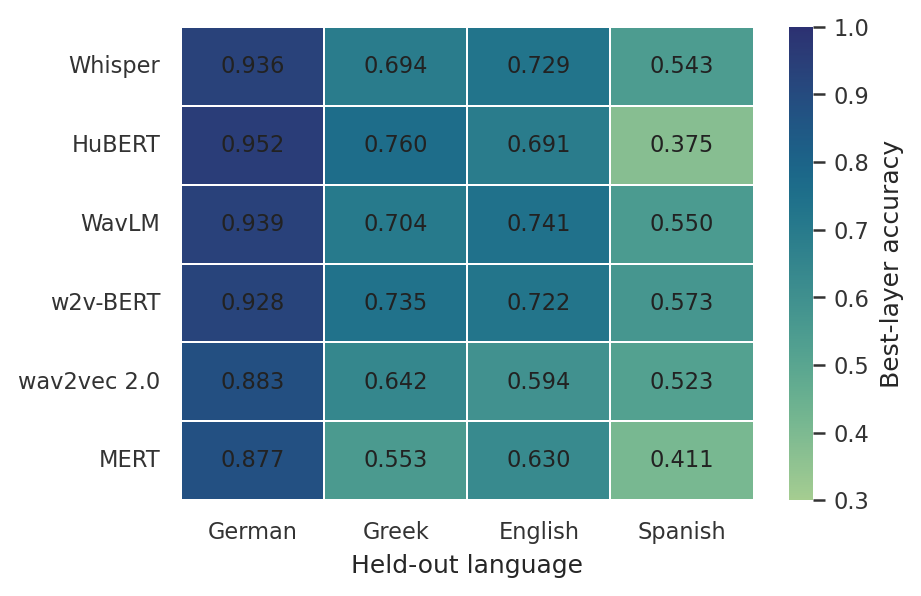
\includegraphics[width=\columnwidth]{speechcraft_lolo_heatmap.png}
\caption{Task 9 Subtask A leave-one-language-out accuracy heatmap. German held out is the easiest condition for every encoder; Spanish held out is the hardest.}
\label{fig:exp20-lolo-heatmap}
\end{figure}
\section{Per-encoder, per-SNR best-layer accuracy (ESC-50 noise)}
\label{app:noise-full}
\begin{table}[h]
\centering
\small
\caption{Best-layer accuracy on MSP-Podcast across the six encoders and four noise levels (Drive: TASK 1/2/8).}
\label{tab:noise-full}
\setlength{\tabcolsep}{4.5pt}
\begin{tabular}{lccccc}
\toprule
\textbf{Encoder} & \textbf{Clean} & \textbf{20\,dB} & \textbf{10\,dB} & \textbf{5\,dB} & \textbf{0\,dB} \\
\midrule
HuBERT       & 0.855 & 0.807 & 0.767 & 0.722 & 0.655 \\
MERT         & 0.816 & 0.706 & 0.652 & 0.614 & 0.574 \\
WavLM        & 0.863 & 0.812 & 0.754 & 0.685 & 0.616 \\
Whisper      & 0.864 & 0.833 & 0.812 & 0.794 & 0.768 \\
w2v-BERT     & 0.841 & 0.792 & 0.760 & 0.732 & 0.695 \\
wav2vec~2.0  & 0.834 & 0.767 & 0.713 & 0.660 & 0.579 \\
\bottomrule
\end{tabular}
\end{table}
\section{V/A/D regression details}
\label{app:vad-full}
\begin{table}[h]
\centering
\small
\caption{Per-target RMSE averaged across the six encoders, on MSP-Podcast at five noise levels (Drive: TASK 10/11).}
\label{tab:vad-target}
\begin{tabular}{lccccc}
\toprule
\textbf{Target} & \textbf{Clean} & \textbf{20\,dB} & \textbf{10\,dB} & \textbf{5\,dB} & \textbf{0\,dB} \\
\midrule
EmoDom (dominance) & 0.699 & 0.710 & 0.718 & 0.725 & 0.735 \\
EmoAct (arousal)   & 0.730 & 0.746 & 0.759 & 0.770 & 0.786 \\
EmoVal (valence)   & 0.881 & 0.897 & 0.908 & 0.917 & 0.929 \\
\bottomrule
\end{tabular}
\end{table}
\end{document}
